\renewcommand{\thechapter}{4}
\chapter{Denoising Theory and Implementation}
\label{ch:DenoisingTheory}

As has been discussed, the performance of double-beta experiments like EXO-200 is partially determined by their energy resolution.  In EXO-200, the energy resolution is limited by the scintillation energy resolution, which in turn is dominated by electronic noise in the APDs.  It is therefore worthwhile to understand and reduce the noise in the scintillation signals.

\begin{figure}
\begin{center}
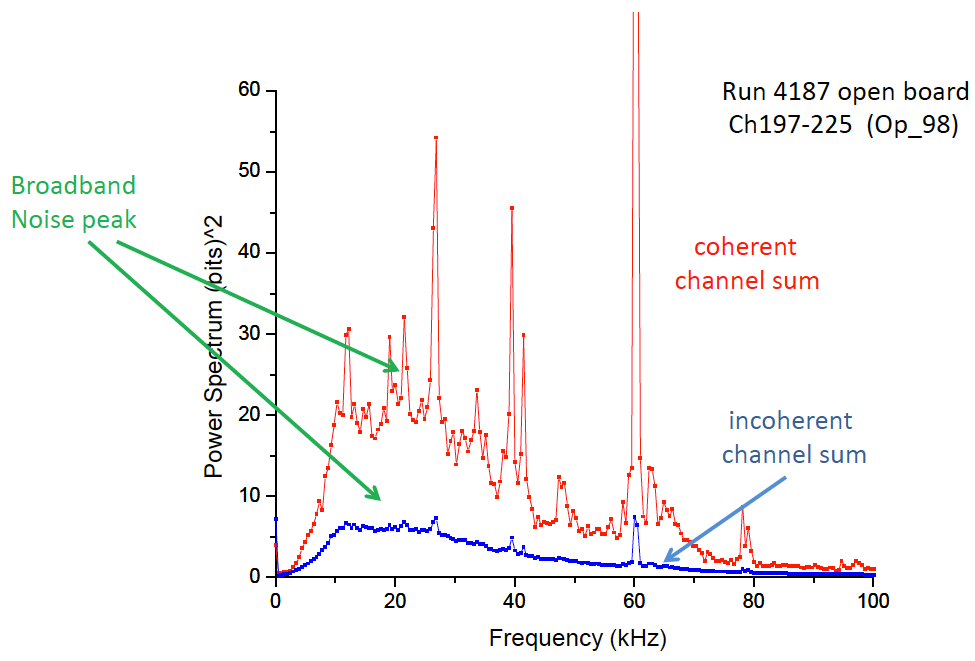
\includegraphics[keepaspectratio=true,width=\textwidth]{APDNoisePowerSpectrum.png}
\end{center}
\renewcommand{\baselinestretch}{1}
\small\normalsize
\begin{quote}
\caption{Coherent and incoherent noise power spectra for a sample set of APD channels without signal shaping~\cite{ElectronicsUpgradeReport}.}
\label{fig:APDNoisePowerSpectrum}
\end{quote}
\end{figure}
\renewcommand{\baselinestretch}{2}
\small\normalsize

When the noise in the APDs is studied, it is found that the individual APD channels meet targeted root-mean-square noise levels of 2000 electrons~\cite{ElectronicsUpgradeReport}.  However, rather than observing the noise on summed APD channels increase proportionally to the square root of the number of channels, the summed APD noise is roughly two to three times higher than projected.  This unfortunate scaling of the noise with channels indicates that noise across different channels is correlated, and further analysis confirms that the bulk of the noise on an unshaped APD waveform is correlated with other channels, as shown in Figure~\ref{fig:APDNoisePowerSpectrum}.  There are many possible sources of coherent noise in the hardware, and reducing the amount of coherent noise is a topic for further research~\cite{ElectronicsUpgradeReport}.

However, since coherent noise is the dominant type of noise in the APDs, and thus also the limiting factor in EXO-200's energy resolution, it should be possible to exploit the correlations and reduce the level of noise in offline analysis.  This chapter describes a scheme to accomplish that goal and produce an optimal estimate of scintillation energy which takes noise correlations into account.

It is worth noting that in fact there are a number of different qualitative approaches to reducing the noise levels in the scintillation channel.  We will refer to ``passive" approaches as those in which components of our signals are weighted based on their relative signal-to-noise content.  ``Active" approaches, by contrast, will be classified as those which attempt to improve the signal-to-noise content of the waveforms.  We identify the following three types of denoising:
\begin{description}
\item[Frequency weighting] \hfill \\
On a given channel signal, weight more heavily the frequency components which contain larger signal-to-noise ratio.  This passive denoising scheme requires knowledge of the power spectra of the signal and the noise.

\item[Channel weighting] \hfill \\
Different channels may have differing levels of noise, so some may generally have higher-quality signals.  More importantly, though, the amount of signal on a given channel depends strongly on the proximity of the APD gang to the source of scintillation within the detector.  This passive denoising scheme therefore allows us to weight more heavily the channels which have more scintillation, provided we can identify these weights on an event-by-event basis.  This requires knowledge of the magnitude of noise on each channel and of the correspondence between event position and signal magnitude on each APD gang. The latter is described by the lightmap, described earlier.

\item[Noise subtraction] \hfill \\
This active form of denoising consists of using correlations between noise on multiple channels to produce a better estimate of the noise component of waveforms than each signal taken independently could provide.  To accomplish this, we require detailed information about the pairwise noise correlations across channels at each frequency.
\end{description}

In the following, we describe a general linear operator on the APD signals which in principle can accomplish each of these forms of denoising, assuming that all of the necessary inputs are available. By identifying the parameters for that linear operator which are optimal, we can be confident that the denoising operator will accomplish all three forms of denoising described above.

\section{Setup}\label{sec:DenoisingNotationSetup}

We first establish a number of notational conventions:
\begin{itemize}
\item $i$, $j$ will represent indices over APD channels.
\item $a$, $b$, $c$ will represent indices of signals in an event.
\item $\tau$ will represent the time indices of a discrete waveform; $t_a$ represents the calendar time of a signal $a$.
\item $f$, $g$ will represent the frequency indices of Fourier-transformed waveforms.
\item For a waveform $*[\tau]$, we will represent the discrete Fourier transform of that waveform with $\widetilde{*}[f]$, where the particular convention used to evaluate the Fourier transform is not significant.
\item For a Fourier-transformed waveform $\widetilde{*}[f]$, we denote the real and imaginary parts of that waveform by $\widetilde{*}^R[f]$ and $\widetilde{*}^I[f]$, respectively.
\item For an unknown parameter $*$, the symbol $\widehat{*}$ will identify an estimator for $*$.
\item For an expression $*$ containing random variables, $\left<*\right>$ is the expectation value of $*$.
\end{itemize}

We describe the data as a collection of discretely sampled waveforms, $X_i[\tau]$.  We assume that all signal times and shapes are already known, so we can model the waveforms by $X_i[\tau] = \sum_a M_{ia}Y_{ia}[\tau] + N_i[\tau] + b_i$, where $Y$ is the shape of signal $a$ on channel $i$, $M$ is the magnitude of that signal, and $N$ and $b$ represent the electronic noise and baseline, respectively, of the channel.

To break the degeneracy between $M$ and $Y$, we choose to fix the magnitude of the template signal $Y$.  We choose to require that the signal $Y$ has a magnitude of one, as described in figure~\ref{fig:SampleAPDTemplates}.  We assume that the expected magnitude of a signal on channel $i$ from a single-site $2615$-keV deposit is known, and is characterized as a function $L_i(\vec{x}, t)$ of the deposit position $\vec{x}$ and calendar time $t$.  The exact methods for measuring $L_i(\vec{x}, t)$ will be described in chapter~\ref{ch:Lightmap}.  In cases where a multi-site event deposits energy in multiple locations, we use the charge information to estimate the energy deposited in each location; the estimated lightmap yield from such an event will be a weighted sum:
\begin{equation}
L_i^{MS}(\vec{x}_1, \dots, \vec{x}_{n_{max}}, t) = \frac{\sum_n E_n^{charge} L_i(\vec{x}_n, t)}{\sum_n E_n^{charge}}.
\end{equation}
For notational simplicity, we will still characterize the expected yield on a gang $i$ from a multi-site event as $L_i(\vec{x}, t)$; in practice it will always be clear how to compute the expected yields for any event from this function.  We can thereby characterize the expected yields $M_{ia}$ from an event with energy $E_a$ as:
\begin{equation}
\left< M_{ia} \right> = L_i(\vec{x}_a, t_a) E_a.
\end{equation}

\begin{figure}
\begin{center}
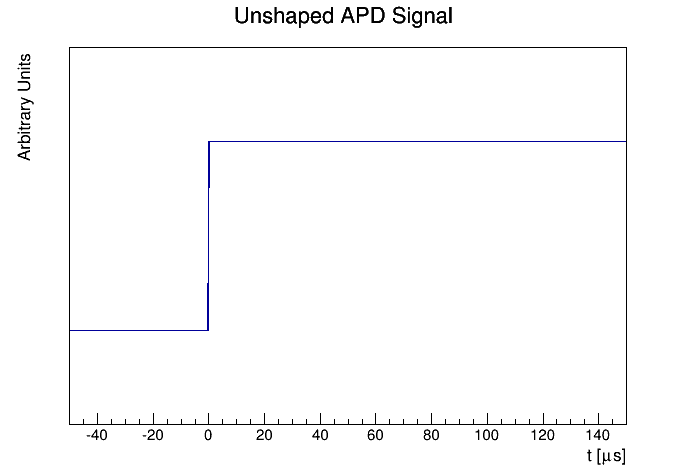
\includegraphics[keepaspectratio=true,width=4in]{scripts/UnshapedAPDWaveform.png}
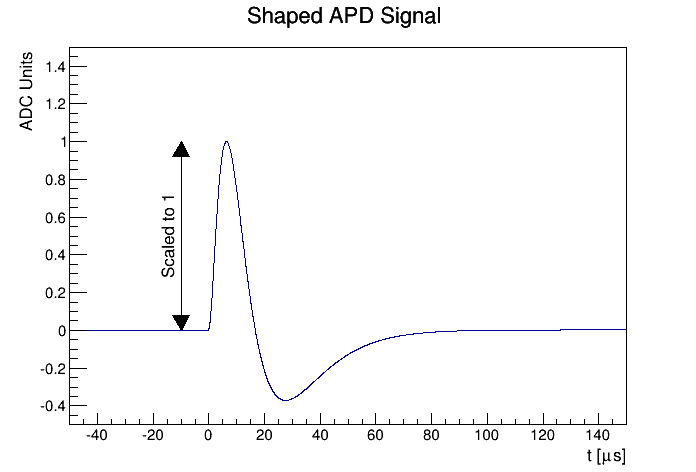
\includegraphics[keepaspectratio=true,width=4in]{scripts/ShapedAPDWaveform.png}
\end{center}
\renewcommand{\baselinestretch}{1}
\small\normalsize
\begin{quote}
\caption{Shaped and unshaped APD waveforms.  The normalization is shown to make the peak of the shaped waveform have a magnitude of one, and the time axis is shifted so that the unshaped waveform is a step function centered at $t=0$.}
\label{fig:SampleAPDTemplates}
\end{quote}
\end{figure}
\renewcommand{\baselinestretch}{2}
\small\normalsize

Noise correlations will be much simpler in frequency space, so we take the Fourier transform and drop the zero-frequency component to obtain
\begin{equation}
\widetilde{X}_i[f] = \sum_a M_{ia}\widetilde{Y}_{ia}[f] + \widetilde{N}_i[f].
\end{equation}
As with the lightmap, we will assume that all correlations in the noise, of the form
\begin{subequations}\begin{align}
&\left< \widetilde{N}^R_i[f]\widetilde{N}^R_j[g] \right> \\
&\left< \widetilde{N}^R_i[f]\widetilde{N}^I_j[g] \right> \\
&\left< \widetilde{N}^I_i[f]\widetilde{N}^R_j[g] \right> \\
&\left< \widetilde{N}^I_i[f]\widetilde{N}^I_j[g] \right>,
\end{align}\end{subequations}
are known; our means of measuring these correlations will be described in chapter~\ref{ch:NoiseMeasurements}.

\section{The Signal Model}

It is important to characterize the response of the APDs to energy deposits in EXO-200.  This requires us to understand the signal amplification of the detector at each physical stage, as well as the noise introduced by each of these processes.  We will describe both in detail here.

\subsection{APD Noise}\label{sec:DescriptionOfPhotonNoise}

We assume that there are two sources of noise in this model.  First, the electronic noise $N_i[\tau]$ is assumed to be random.  We require that noise with different frequencies is uncorrelated:
\begin{equation}\label{eq:FirstStatementOfNoiseCorrelations}
\left< \widetilde{N}_i[f] \widetilde{N}_j[g] \right> = 0 \text{~when~} f \ne g.
\end{equation}
The noise correlations $\left< \widetilde{N}_i[f] \widetilde{N}_j[f] \right>$ are assumed to be known; our means for measuring them are described in chapter~\ref{ch:NoiseMeasurements}.

The second random variable will be the magnitude of the signal itself, $M_{ia}$.  When an energetic decay occurs in the bulk of the detector, it creates some number of photons.  We will denote the number of photons created by signal $a$ by $P^{(0)}_a$, and this is the parameter we wish to measure.  However, the magnitude of the signal actually observed on APD channels number of photons actually collected by sensors is a random variable whose distribution depends on $P^{(0)}_a$, and we will now identify the chain of events which produce it.

First, each APD gang $i$ has some number $P^{(1)}_{ia}$ of photons which reach them.  The mean fraction of photons reaching a particular gang $i$ from position $\vec{x}_a$, $f_i(\vec{x}_a)$, is assumed to be known; however, the initial paths of the optical photons emitted from the source, their trajectories through the Xenon, and their success in reflecting off of teflon are all random, so we treat $P^{(1)}_{ia}$ as a Poisson-distributed random variable with mean $f_i(\vec{x}_a)P^{(0)}_a$.  A typical $\beta\beta 0\nu$ event may deposit up to roughly $1000$ photons on a nearby APD gang, resulting in roughly $3\%$ uncertainty from photon statistics; in the bulk of the Xenon, it may be that the largest single APD signal is only one-tenth of this size, resulting in closer to $10\%$ uncertainty due to photon statistics on the nearest APD gang.  Thus, we find that the Poisson noise on a single APD channel may be quite significant.

Additionally, the number of photons reaching different gangs are not uncorrelated; since a photon which reaches gang $i$ cannot deposit on a different gang $j$, $P^{(1)}_{ia}$ and $P^{(1)}_{ja}$ are anticorrelated for different gangs $i \ne j$.  This process is described by a multinomial distribution.  Explicitly, the expectation values of a multinomial distribution:
\begin{IEEEeqnarray}{cCl}
\left< P^{(1)}_{ia} \right> &=& f_i(\vec{x}_a)P^{(0)}_a \IEEEyesnumber\IEEEyessubnumber\label{eqn:MeanOfP1}\\
\left< P^{(1)}_{ia} P^{(1)}_{jb} \right> &=& \left< P^{(1)}_{ia} \right> \left< P^{(1)}_{jb} \right> + \left[ f_i(\vec{x}_a)\delta_{ij} - f_i(\vec{x}_a)f_j(\vec{x}_a) \right] P^{(0)}_a \delta_{ab} \IEEEyessubnumber
\end{IEEEeqnarray}

(As a detail, we should note that the multinomial distribution is an incorrect model in one important respect: photons may reflect off of teflon one or more times on its way to the APD.  Photons incident on the teflon may be absorbed, leading to a reflection efficiency which may be less than one.  Furthermore, it is possible that teflon may be mildly fluorescent at the wavelength of our scintillation, leading to an increase in efficiency for reflection.  As a result, photons which reflect off of teflon experience a combination of variances from each path photons travel and variances in each gain which they undergo.  These conditional variances will always be larger than a simple Poisson distribution would indicate~\cite{ProbabilityTextbook}, so our variance estimate for $P^{(1)}$ is probably an underestimate.)

Following the random process associated with photons reaching the APD gangs, there is also randomness associated with signal amplification internally in the APDs.  These processes are described in detail in~\cite{EXOLAAPD}, but we summarize here:

\begin{enumerate}
\item Scintillation photons arrive at the active layer of the APDs. The energy required to produce one electron-hole pair in silicon is $3.66$ eV, so each incident photon produces roughly $1.9$ electron-hole pairs. We will define $P^{(2)}_{ia}$ to be the number of electron-hole pairs actually produced from $P^{(1)}_{ia}$ incident photons.  The corresponding Fano factor for electrons produced in silicon is roughly $0.1$, meaning that in addition to the uncertainty in $P^{(1)}_{ia}$ which we have already characterized, there is an additional uncorrelated variance in $P^{(2)}_{ia}$ equal to $0.1 \left<P^{(2)}_{ia}\right>$.  The correlations in the parameters $P^{(2)}_{ia}$ are therefore:
\begin{IEEEeqnarray}{cCl}
\left< P^{(2)}_{ia} \right> &=& 1.9 \cdot P^{(1)}_{ia} \IEEEyesnumber\IEEEyessubnumber \label{eqn:MeanOfP2}\\
\left< P^{(2)}_{ia} P^{(2)}_{jb} \right> &=& (1.9)^2\left< P^{(1)}_{ia} P^{(1)}_{jb} \right> + 0.1 \left< P^{(2)}_{ia}\right> \delta_{ij}\delta_{ab} \IEEEyessubnumber \label{eqn:VarOfP2}
\end{IEEEeqnarray}
\item Electron-hole pairs are then amplified by an avalanche process inside the APDs.  The magnitude of this gain is APD-dependent, generally on the order of $200-300$, and can be identified by a time-dependent quantity $G^P_i(t)$; we will call the number of output electrons $P^{(3)}_{ia}$.  In addition to amplification of existing noise in $P^{(2)}_{ia}$, two additional source of noise are introduced.  First, there is statistical variance in the amplification experienced by each electron due to the randomness of the avalanche process.  This variance is dependent on many factors, including the gain, and scales like the square root of the number of electrons; we define the variance on the gain experienced by a single electron as $\sigma^2_{G_i}(t)$.  From~\cite{EXOLAAPD}, $\sigma^2_{G_i}(t)$ is approximately equal to $\left(G^P_i(t)\right)^2$ when $G^P_i(t)=100$; as a result, we approximate $\sigma^2_{G_i}(t) \approx \left(G^P_i(t)\right)^2$.  Second, there are gain non-uniformities in the diode volume, which contribute variance proportional to the square of the number of initial electron-hole pairs; we will identify the proportionality constant as $\sigma^2_{NU}$, which may depend on time and APD gang.  The magnitude of this uncertainty is not well-known, but may be significant.  Our current code base treats $\sigma^2_{NU}$ as zero; however, future analyses will likely attempt to estimate it, and the derivation which follows will retain it as an aid to that anticipated work.  The correlations in the parameters $P^{(3)}_{ia}$ are therefore:
\begin{IEEEeqnarray}{cCl}
\left< P^{(3)}_{ia} \right> &=& G^P_i(t_a)P^{(2)}_{ia} \IEEEyesnumber\IEEEyessubnumber \label{eqn:MeanOfP3}\\
\left< P^{(3)}_{ia} P^{(3)}_{jb} \right> &=& G^P_i(t_a)G^P_j(t_b) \left< P^{(2)}_{ia} P^{(2)}_{jb} \right> + \left[P^{(2)}_{ia}\sigma^2_{G_i}(t_a) + \left(P^{(2)}_{ia}\right)^2\sigma^2_{NU}\right]\delta_{ij}\delta_{ab} \nonumber \\* \IEEEyessubnumber\label{eqn:VarOfP3}
\end{IEEEeqnarray}
\end{enumerate}

\textcolor{red}{My thinking on non-uniformities has evolved a little bit -- clarify in this section why it's such a big deal.}

Finally, there is amplification
\begin{equation} \label{eqn:DefnOfMFromP3}
M_{ia} = G^{E}_i(t) P^{(3)}_{ia}
\end{equation}
associated with the electronics of the APDs which is dependent on time and channel.  This includes preamplifier gain, shaper gain, gain associated with the shaping times, and conversion from voltage to ADC counts.  We assume that no signal-dependent noise is introduced during this stage, but there is constant electronic noise $N_i[\tau]$ which has been described above.  Additionally, the APDs can contribute noise in the form of a dark current which is uncorrelated with signals; this is inseparable from the electronic noise, and so we absorb it into our description of $N_i[\tau]$.

\subsection{APD Signals and Noise}

We have characterized the overall gain of the APDs using the lightmap described earlier.  We know that a typical single-site deposit of $2615$ keV at position $\vec{x}$ and time $t$ will produce a signal with expected magnitude $L_i(\vec{x},t)$ on APD channel $i$.  We must now connect this empirical understanding of our APD signals with the physical understanding in terms of photons and electrons described above.

We have identified the number of photons created by an event $a$ as $P^{(0)}_a$.  In reality, an ideal scintillation measurement can only measure this quantity, and not the true energy of the event -- there is randomness in the number of photons produced by a known-energy deposit, so $P^{(0)}_a$ will not be a perfect measure of the energy $E_a$ of the event.  However, the number of photons generated is a difficult parameter to understand empirically, and all of our calibrations occur at a known energy even though the corresponding number of deposited photons is unknown.

Simulations using NEST~\cite{NESTpaper} which have been performed within the EXO group by Liangjian Wen at our bulk electric field indicate that we can expect $82,000$ photons from a $2615$-keV gamma deposit.  We will identify this parameter with $c$, and express the average relation between energy and photon yield in EXO-200 by
\begin{equation} \label{eqn:DefnOfP0}
P^{(0)} = c \cdot E,
\end{equation}
where $E$ is the energy measured in units of $2615$ keV.  We will treat this relationship as exact, and attempt to measure $E$ rather than $P^{(0)}$; this means that when we speak of measuring the energy of an event using the APD signals, we really are referring to measuring the ``scintillation energy," or a parameter proportional to the number of emitted photons which on average will equal the true energy of the deposit.

Ignoring variances for a moment, we can combine equations~\ref{eqn:MeanOfP1}, \ref{eqn:MeanOfP2}, \ref{eqn:MeanOfP3}, \ref{eqn:DefnOfMFromP3}, and \ref{eqn:DefnOfP0} to state that on average,
\begin{equation}
M_{ia} = 1.9 \cdot c f_i(\vec{x}_a) G^P_i(t_a) G^E_i(t_a) E_a.
\end{equation}
We can compare this to our empirical lightmap measurements, which are expressed by $M_{ia} = L_i(\vec{x}_a,t_a) E_a$,
and we conclude that:
\begin{equation}
L_i(\vec{x},t) = 1.9 \cdot c f_i(\vec{x}) G^P_i(t) G^E_i(t).
\end{equation}

We recall that it is assumed the lightmap is a separable function, $L_i(\vec{x},t) = R_i(\vec{x})S_i(t)$, and we can provide the two proportionalities:
\begin{subequations}\begin{align}
R_i(\vec{x}) &\propto f_i(\vec{x}) \\
S_i(t) &\propto G^P_i(t) G^E_i(t).
\end{align}\end{subequations}

Although $G^E_i(t)$ is in principle time-dependent, due to environmental effects on the APD electronics and occasional replacement of electronics cards for certain channels, precision data on its value is not readily available.  Instead, we use a time-independent estimate
\begin{equation}
G^E_i(t) = 1.1 \cdot 10^{-3} \label{eqn:ValueOfGE}
\end{equation}
ADC counts per electron emitted from the APD; the uncertainty in this figure is dominated by uncertainty in the preamplifier gains, which are controlled by a $5$ pF capacitor.  Other contributors to the gain include shaper gain of $21.2$ (from a combination of amplification and shaping) and a full-scale digitizer range of $2.5$ volts for $12$-bit digitization.

We have independent measurements of the APD gains $G^P_i(t)$ available from laser calibration runs.  These special runs allow a laser to shine into the detector from a fixed point and with a stable amplitude while the bias voltages on the APDs are varied from an effective unity gain to our standard voltage settings.  Using these measurements, we are able to measure $G^P_i(t)$ at weekly intervals from September 2012 to the present time.  Before September 2012, some less-reliable laser data is available, but results from that data are not readily available as of this writing.

It would be possible, and should be a goal for future improvements, to make use of this full range of laser data.  However, the laser data provides a less uniform history of APD gains over the full data-taking window of EXO-200 from September 2011 to November 2013, and it is much easier to track time-dependent behavior from Thorium source data which have been collected regularly throughout that period.  As a result, a compromise is used to characterize $G^P_i(t)$.  One particular laser run, run 4540 (taken on December 13, 2012), is used to fix $G^P_i(t_{4540})$, and the function is extrapolated using Thorium source data with:
\begin{equation}
G^P_i(t) \approx G^P_i(t_{4540}) \cdot S_i(t)/S_i(t_{4540}).
\end{equation}
This assumption makes use of the approximation that $G^E_i(t)$ is roughly constant in time, which is probably only accurate to one significant figure; therefore when an electronics change is made to a channel, we can expect that the accuracy of $G^P_i(t)$ is no better than one significant figure.  These results mean that we can also estimate with the same level of accuracy:
\begin{equation}
f_i(\vec{x}) \approx \frac{S_i(t_{4540})}{G^P_i(t_{4540})} \cdot \frac{R_i(\vec{x})}{1.9 \cdot c G^E_i(t)}.
\end{equation}

It is then possible to express the full correlations in signal magnitudes in terms of the scintillation energies of deposits as:
\begin{IEEEeqnarray}{cCl}
\left< M_{ia} \right> &=& L_i(\vec{x}_a,t_a) E_a \IEEEyesnumber\IEEEyessubnumber \\
\left< M_{ia} M_{jb} \right> &=& L_i(\vec{x}_a,t_a)L_j(\vec{x}_b,t_b) E_a E_b \left[1 + \frac{\sigma^2_{NU}}{\left(G^P_i(t)\right)^2} \delta_{ij}\delta_{ab} \right] \nonumber \\
&& {} - L_i(\vec{x}_a,t_a) L_j(\vec{x}_a,t_a) E_a \delta_{ab}/c \nonumber \\
&& {} + L_i(\vec{x}_a,t_a) G^E_i(t) E_a \delta_{ij} \delta_{ab} \left[\left(0.1 + 1.9\right)G^P_i(t) + \frac{\sigma^2_{G_i}(t)}{G^P_i(t)}\right]. \IEEEyessubnumber\label{eqn:MMcorrelations}
\end{IEEEeqnarray}
\begin{comment}
THE FOLLOWING IS MY WORK IN EXPANDING THE M_M CORRELATIONS.
IF NEEDED, IT CAN BE UNCOMMENTED AND IS VALID LATEX CODE.

\[ \left< M_{ia} M_{jb} \right> = G^E_i(t) G^E_j(t) \left<P^{(3)}_{ia}P^{(3)}_{jb} \right> \]

\[ \left< M_{ia} M_{jb} \right> = G^E_i(t) G^E_j(t) \left( G^P_i(t)G^P_j(t) \left< P^{(2)}_{ia} P^{(2)}_{jb} \right> + \left[P^{(2)}_{ia}\sigma^2_{G_i}(t) + \left(P^{(2)}_{ia}\right)^2\sigma^2_{NU}\right]\delta_{ij}\delta_{ab}\right)\]

\begin{equation*}\begin{split}
\left< M_{ia} M_{jb} \right> ={}& G^E_i(t) G^E_j(t) G^P_i(t)G^P_j(t) \left< P^{(2)}_{ia} P^{(2)}_{jb} \right> \\
 & + G^E_i(t) G^E_j(t) \left[P^{(2)}_{ia}\sigma^2_{G_i}(t) + \left(P^{(2)}_{ia}\right)^2\sigma^2_{NU}\right]\delta_{ij}\delta_{ab}
\end{split}\end{equation*}

\begin{equation*}\begin{split}
\left< M_{ia} M_{jb} \right> ={}& G^E_i(t) G^E_j(t) G^P_i(t)G^P_j(t) \left( (1.9)^2\left< P^{(1)}_{ia} P^{(1)}_{jb} \right> + 0.1 \left< P^{(2)}_{ia}\right> \delta_{ij}\delta_{ab} \right) \\
 & + G^E_i(t) G^E_j(t) \left[1.9 \cdot P^{(1)}_{ia}\sigma^2_{G_i}(t) + (1.9)^2 \left(P^{(1)}_{ia}\right)^2\sigma^2_{NU}\right]\delta_{ij}\delta_{ab}
\end{split}\end{equation*}

\begin{equation*}\begin{split}
\left< M_{ia} M_{jb} \right> ={}& (1.9)^2 G^E_i(t) G^E_j(t) G^P_i(t)G^P_j(t) \left< P^{(1)}_{ia} P^{(1)}_{jb} \right> \\
& + 0.1 \cdot 1.9 \cdot G^E_i(t) G^E_j(t) G^P_i(t)G^P_j(t) P^{(1)}_{ia} \delta_{ij}\delta_{ab} \\
 & + G^E_i(t) G^E_j(t) \left[1.9 \cdot P^{(1)}_{ia}\sigma^2_{G_i}(t) + (1.9)^2 \left(P^{(1)}_{ia}\right)^2\sigma^2_{NU}\right]\delta_{ij}\delta_{ab}
\end{split}\end{equation*}

\begin{equation*}\begin{split}
\left< M_{ia} M_{jb} \right> ={}& (1.9)^2 G^E_i(t) G^E_j(t) G^P_i(t)G^P_j(t) \left< P^{(1)}_{ia} P^{(1)}_{jb} \right> \\
 & + G^E_i(t) G^E_j(t) \left[1.9 \cdot P^{(1)}_{ia}\sigma^2_{G_i}(t) + (1.9)^2 \left(P^{(1)}_{ia}\right)^2\sigma^2_{NU} + 0.1 \cdot 1.9 \cdot G^P_i(t)G^P_j(t) P^{(1)}_{ia}\right]\delta_{ij}\delta_{ab}
\end{split}\end{equation*}

\begin{equation*}\begin{split}
\left< M_{ia} M_{jb} \right> ={}& (1.9)^2 G^E_i(t) G^E_j(t) G^P_i(t)G^P_j(t) \left< P^{(1)}_{ia} P^{(1)}_{jb} \right> \\
 & + 1.9\left[\sigma^2_{G_i}(t) + 1.9 \cdot P^{(1)}_{ia} \sigma^2_{NU} + 0.1 \cdot G^P_i(t)G^P_j(t) \right] \left(G^E_i(t)\right)^2 P^{(1)}_{ia} \delta_{ij}\delta_{ab}
\end{split}\end{equation*}

\begin{equation*}\begin{split}
\left< M_{ia} M_{jb} \right> ={}& (1.9)^2 G^E_i(t) G^E_j(t) G^P_i(t)G^P_j(t) \left< P^{(1)}_{ia} \right> \left< P^{(1)}_{jb} \right> \\
& + (1.9)^2 G^E_i(t) G^E_j(t) G^P_i(t)G^P_j(t)\left[ f_i(x,y,z)\delta_{ij} - f_i(x,y,z)f_j(x,y,z) \right] P^{(0)}_a \delta_{ab}  \\
 & + 1.9\left[\sigma^2_{G_i}(t) + 1.9 \cdot P^{(1)}_{ia} \sigma^2_{NU} + 0.1 \cdot G^P_i(t)G^P_j(t) \right] \left(G^E_i(t)\right)^2 P^{(1)}_{ia} \delta_{ij}\delta_{ab}
\end{split}\end{equation*}

\begin{equation*}\begin{split}
\left< M_{ia} M_{jb} \right> ={}& (1.9)^2 G^E_i(t) G^E_j(t) G^P_i(t)G^P_j(t) f_i(x,y,z) f_j(x,y,z) \left(P^{(0)}_a\right)^2 \\
& + (1.9)^2 G^E_i(t) G^E_j(t) G^P_i(t)G^P_j(t)\left[ f_i(x,y,z)\delta_{ij} - f_i(x,y,z)f_j(x,y,z) \right] P^{(0)}_a \delta_{ab}  \\
 & + 1.9\left[\sigma^2_{G_i}(t) + 1.9 \cdot f_i(x,y,z) P^{(0)}_a \sigma^2_{NU} + 0.1 \cdot G^P_i(t)G^P_j(t) \right] \left(G^E_i(t)\right)^2 f_i(x,y,z) P^{(0)}_a \delta_{ij}\delta_{ab}
\end{split}\end{equation*}

\begin{equation*}\begin{split}
\left< M_{ia} M_{jb} \right> ={}& (1.9)^2 G^E_i(t) G^E_j(t) G^P_i(t)G^P_j(t) f_i(x,y,z) f_j(x,y,z) c^2 E^2_a \\
& + (1.9)^2 G^E_i(t) G^E_j(t) G^P_i(t)G^P_j(t)\left[ f_i(x,y,z)\delta_{ij} - f_i(x,y,z)f_j(x,y,z) \right] c E_a \delta_{ab}  \\
 & + 1.9\left[\sigma^2_{G_i}(t) + 1.9 \cdot f_i(x,y,z) c E_a \sigma^2_{NU} + 0.1 \cdot G^P_i(t)G^P_j(t) \right] \left(G^E_i(t)\right)^2 f_i(x,y,z) c E_a \delta_{ij}\delta_{ab}
\end{split}\end{equation*}

\begin{equation*}\begin{split}
\left< M_{ia} M_{jb} \right> ={}& L_i(x,y,z,t)L_j(x,y,z,t) E^2_a \\
& + (1.9)^2 G^E_i(t) G^E_j(t) G^P_i(t)G^P_j(t) f_i(x,y,z)\delta_{ij} c E_a \delta_{ab}  \\
& - (1.9)^2 G^E_i(t) G^E_j(t) G^P_i(t)G^P_j(t) f_i(x,y,z)f_j(x,y,z) c E_a \delta_{ab} \\
 & + 1.9\left[\sigma^2_{G_i}(t) + 1.9 \cdot f_i(x,y,z) c E_a \sigma^2_{NU} + 0.1 \cdot G^P_i(t)G^P_j(t) \right] \left(G^E_i(t)\right)^2 f_i(x,y,z) c E_a \delta_{ij}\delta_{ab}
\end{split}\end{equation*}

\begin{equation*}\begin{split}
\left< M_{ia} M_{jb} \right> ={}& L_i(x,y,z,t)L_j(x,y,z,t) E^2_a \\
& + L_i(x,y,z,t) (1.9)  G^E_i(t) G^P_i(t) \delta_{ij}  E_a \delta_{ab}  \\
& - L_i(x,y,z,t)     (1.9) G^E_j(t) G^P_j(t) f_j(x,y,z) E_a \delta_{ab} \\
 & + 1.9\left[\sigma^2_{G_i}(t) + 1.9 \cdot f_i(x,y,z) c E_a \sigma^2_{NU} + 0.1 \cdot \left(G^P_i(t)\right)^2 \right] \left(G^E_i(t)\right)^2 f_i(x,y,z) c E_a \delta_{ij}\delta_{ab}
\end{split}\end{equation*}

\begin{equation*}\begin{split}
\left< M_{ia} M_{jb} \right> ={}& L_i(x,y,z,t)L_j(x,y,z,t) E^2_a \\
& + L_i(x,y,z,t) (1.9)  G^E_i(t) G^P_i(t) E_a \delta_{ij} \delta_{ab}  \\
& - L_i(x,y,z,t) L_j(x,y,z,t) E_a \delta_{ab}/c \\
& + (1.9)\sigma^2_{G_i}(t)\left(G^E_i(t)\right)^2 f_i(x,y,z) c E_a \delta_{ij}\delta_{ab} \\
& + (1.9)^2 f_i(x,y,z) c E_a \sigma^2_{NU} \left(G^E_i(t)\right)^2 f_i(x,y,z) c E_a \delta_{ij}\delta_{ab} \\
& + (1.9) (0.1) \left(G^P_i(t)\right)^2 \left(G^E_i(t)\right)^2 f_i(x,y,z) c E_a \delta_{ij}\delta_{ab}
\end{split}\end{equation*}

\begin{equation*}\begin{split}
\left< M_{ia} M_{jb} \right> ={}& L_i(x,y,z,t)L_j(x,y,z,t) E^2_a \\
& + (1.9)^2 f^2_i(x,y,z) \sigma^2_{NU} \left(G^E_i(t)\right)^2 c^2 E^2_a \delta_{ij}\delta_{ab} \\
& - L_i(x,y,z,t) L_j(x,y,z,t) E_a \delta_{ab}/c \\
& + L_i(x,y,z,t) (1.9)  G^E_i(t) G^P_i(t) E_a \delta_{ij} \delta_{ab}  \\
& + (1.9)\sigma^2_{G_i}(t)\left(G^E_i(t)\right)^2 f_i(x,y,z) c E_a \delta_{ij}\delta_{ab} \\
& + L_i(x,y,z,t) (0.1) G^P_i(t) G^E_i(t) E_a \delta_{ij}\delta_{ab}
\end{split}\end{equation*}

\begin{equation*}\begin{split}
\left< M_{ia} M_{jb} \right> ={}& L_i(x,y,z,t)L_j(x,y,z,t) E^2_a \\
& + L^2_i(x,y,z,t) \sigma^2_{NU} E^2_a \delta_{ij}\delta_{ab}/\left(G^P_i(t)\right)^2 \\
& - L_i(x,y,z,t) L_j(x,y,z,t) E_a \delta_{ab}/c \\
& + L_i(x,y,z,t) (1.9)  G^E_i(t) G^P_i(t) E_a \delta_{ij} \delta_{ab}  \\
& + L_i(x,y,z,t) \sigma^2_{G_i}(t)G^E_i(t) E_a \delta_{ij}\delta_{ab}/G^P_i(t) \\
& + L_i(x,y,z,t) (0.1) G^P_i(t) G^E_i(t) E_a \delta_{ij}\delta_{ab}
\end{split}\end{equation*}

\begin{equation*}\begin{split}
\left< M_{ia} M_{jb} \right> ={}& L_i(x,y,z,t)L_j(x,y,z,t) E^2_a \left[1 + \frac{\sigma^2_{NU}}{\left(G^P_i(t)\right)^2} \delta_{ij}\delta_{ab} \right] \\
& - L_i(x,y,z,t) L_j(x,y,z,t) E_a \delta_{ab}/c \\
& + L_i(x,y,z,t) \sigma^2_{G_i}(t)G^E_i(t) E_a \delta_{ij}\delta_{ab}/G^P_i(t) \\
& + L_i(x,y,z,t) (1.9 + 0.1)  G^E_i(t) G^P_i(t) E_a \delta_{ij} \delta_{ab}
\end{split}\end{equation*}

\begin{equation*}\begin{split}
\left< M_{ia} M_{jb} \right> ={}& L_i(x,y,z,t)L_j(x,y,z,t) E^2_a \left[1 + \frac{\sigma^2_{NU}}{\left(G^P_i(t)\right)^2} \delta_{ij}\delta_{ab} \right] \\
& - L_i(x,y,z,t) L_j(x,y,z,t) E_a \delta_{ab}/c \\
& + L_i(x,y,z,t) G^E_i(t) E_a \delta_{ij} \delta_{ab} \left[\left(0.1 + 1.9\right)G^P_i(t) + \frac{\sigma^2_{G_i}(t)}{G^P_i(t)}\right]
\end{split}\end{equation*}
\end{comment}

We combine this with our knowledge of the noise coefficients:
\begin{subequations}\begin{align}
\left< \widetilde{N}_i[f] \right> &= 0 \\
\left< \widetilde{N}_i[f] \widetilde{N}_j[g] \right> &= \left\{ \begin{aligned}
0~ &\text{if}~ f \ne g \\
\text{known}~ &\text{if}~ f = g
\end{aligned}\right.
\end{align}\end{subequations}
and can claim to now have a complete description of the signals and noise observed in the APD channels.

\section{Derivation}

It is now possible to specify the optimization criteria for generating an energy estimate from the APD signals.  We wish to identify an energy estimator which is unbiased and has a minimal expected error.  For the problem to remain tractable, we will demand that the operator be linear.  Furthermore, although the Fourier-transformed waveforms $\widetilde{X}_i[f]$ are complex-valued, we will require that the energy estimate be strictly real-valued.

We will therefore take the energy estimator to be of the form:
\begin{equation}
\widehat{E}_a = \sum_{if} A_{ifa} \widetilde{X}_i^R[f] + B_{ifa} \widetilde{X}_i^I[f].
\end{equation}
The goal of denoising is therefore reduced to identifying the optimal parameters $A_{ifa}$ and $B_{ifa}$ for this estimator.

The error in the energy estimate $\widehat{E}_a$ of $E_a$ is defined by:
\begin{equation}
\epsilon^2_a = \left< \left(\widehat{E}_a - E_a\right)^2\right>.
\end{equation}
Our goal is to minimize $\epsilon^2_a$ under the constraint of no bias, ie. that:
\begin{equation}\label{eqn:ConstraintForm1}
\left<\widehat{E}_a - E_a\right> = 0
\end{equation}
or, equivalently,
\begin{equation}
\sum_{ifb}\left[A_{ifa} \widetilde{Y}_{ib}^R[f] + B_{ifa} \widetilde{Y}_{ib}^I[f]\right] L_i(\vec{x}_b,t_b) E_b = E_a.
\end{equation}
However, we will find that it is necessary to specify a slightly stronger constraint.  In particular, it will be desirable to ensure that the constraints are as independent of energy as possible to reduce the need to input an estimated energy into our energy estimator; therefore we will freely employ the stronger constraint
\begin{equation}
\sum_{if}\left[A_{ifa} \widetilde{Y}_{ib}^R[f] + B_{ifa} \widetilde{Y}_{ib}^I[f]\right] L_i(\vec{x}_b,t_b) = \delta_{ab} \text{~for all b,} \label{eqn:ConstraintForm3}
\end{equation}
which implies the earlier forms and leads to advantageous cancellations of terms.

We now proceed with the optimization.  We start by expanding $\epsilon^2_a$:
\begin{align}
\epsilon^2_a &= \left< \left(\widehat{E}_a - E_a\right)^2\right> \\
%
&= \left< \widehat{E}^2_a \right> - E_a \left<\widehat{E}_a\right> - \left< \widehat{E}_a - E_a \right> E_a \\
%
\intertext{We can employ the constraint of equation~\ref{eqn:ConstraintForm1} to simplify the second term of this expansion, and eliminate the third altogether; we then proceed:}
%
\epsilon^2_a &= \left< \widehat{E}^2_a \right> - E^2_a \\
%
&= \left< \left(\sum_{if}\left[ A_{ifa} \widetilde{X}_i^R[f] + B_{ifa} \widetilde{X}_i^I[f]\right]\right)^2\right> - E^2_a \\
%
& \begin{aligned}= \bigg< \bigg(&
  \sum_{if} \left[ A_{ifa} \widetilde{N}_i^R[f] + B_{ifa} \widetilde{N}_i^I[f]\right] \\
  & + \sum_{ifb} \left[ A_{ifa} \widetilde{Y}_{ib}^R[f] + B_{ifa} \widetilde{Y}_{ib}^I[f]\right]M_{ib}  \bigg)^2 \bigg> - E^2_a
\end{aligned} \\
%
\intertext{The noise $\widetilde{N}$ and signal $M_{ia}$ are uncorrelated, so multiplicative cross-terms will have an expectation value of zero:}
%
\epsilon^2_a &= \left< \left(\sum_{if} \left[ A_{ifa} \widetilde{N}_i^R[f] + B_{ifa} \widetilde{N}_i^I[f]\right]\right)^2\right> \nonumber \\
&\quad + \left<\left(\sum_{ifb} \left[ A_{ifa} \widetilde{Y}_{ib}^R[f] + B_{ifa} \widetilde{Y}_{ib}^I[f]\right]M_{ib} \right)^2 \right> - E^2_a \\
%
\intertext{Additionally, electronic noise cross-terms between different frequencies will not survive:}
%
\epsilon^2_a &= \left< \sum_{ijf} \left[ A_{ifa} \widetilde{N}_i^R[f] + B_{ifa} \widetilde{N}_i^I[f]\right] \left[ A_{jfa} \widetilde{N}_j^R[f] + B_{jfa} \widetilde{N}_j^I[f]\right] \right> \nonumber \\
&\quad + \left<\left(\sum_{ifb} \left[ A_{ifa} \widetilde{Y}_{ib}^R[f] + B_{ifa} \widetilde{Y}_{ib}^I[f]\right]M_{ib} \right)^2 \right> - E^2_a \\
%
& \begin{aligned}
  = \sum_{ijf} \bigg[ & A_{ifa}A_{jfa} \left<\widetilde{N}_i^R[f]\widetilde{N}_j^R[f]\right> + A_{ifa}B_{jfa} \left<\widetilde{N}_i^R[f]\widetilde{N}_j^I[f]\right> \nonumber \\
  & + B_{ifa}A_{jfa} \left<\widetilde{N}_i^I[f]\widetilde{N}_j^R[f]\right> + B_{ifa}B_{jfa} \left<\widetilde{N}_i^I[f]\widetilde{N}_j^I[f]\right>\bigg] \end{aligned} \nonumber \\
&\quad + \sum_{\substack{ifb\\jgc}} \left[A_{ifa} \widetilde{Y}_{ib}^R[f] + B_{ifa} \widetilde{Y}_{ib}^I[f]\right]\left[A_{jga} \widetilde{Y}_{jc}^R[g] + B_{jga} \widetilde{Y}_{jc}^I[g]\right] \left<M_{ib}M_{jc}\right> - E^2_a \\
%
\intertext{We will now expand $\left<M_{ib}M_{jc}\right>$ using equation~\ref{eqn:MMcorrelations} and take advantage of the stronger form of our constraint~\ref{eqn:ConstraintForm3} to simplify the expression:}
%
\epsilon^2_a & \begin{aligned}[t]
  = \sum_{ijf} \bigg[ & A_{ifa}A_{jfa} \left<\widetilde{N}_i^R[f]\widetilde{N}_j^R[f]\right> + A_{ifa}B_{jfa} \left<\widetilde{N}_i^R[f]\widetilde{N}_j^I[f]\right> \\
  & + B_{ifa}A_{jfa} \left<\widetilde{N}_i^I[f]\widetilde{N}_j^R[f]\right> + B_{ifa}B_{jfa} \left<\widetilde{N}_i^I[f]\widetilde{N}_j^I[f]\right>\bigg] \end{aligned} \nonumber \\
&\quad + \left( \sum_{ifb} \left[A_{ifa} \widetilde{Y}_{ib}^R[f] + B_{ifa} \widetilde{Y}_{ib}^I[f]\right] L_i(\vec{x}_b,t_b) E_b \right)^2 - E^2_a \nonumber \\
&\quad - \sum_b \left( \sum_{if} \left[A_{ifa} \widetilde{Y}_{ib}^R[f] + B_{ifa} \widetilde{Y}_{ib}^I[f]\right] L_i(\vec{x}_b,t_b) \right)^2 \frac{E_b}{c} \nonumber \\
&\quad \begin{aligned}
  + \sum_{ifgb} &\left[A_{ifa} \widetilde{Y}_{ib}^R[f] + B_{ifa} \widetilde{Y}_{ib}^I[f]\right]\left[A_{iga} \widetilde{Y}_{ib}^R[g] + B_{iga} \widetilde{Y}_{ib}^I[g]\right] \cdot \\
  & \begin{aligned}
    L_i(\vec{x}_b,t_b) E_b \bigg[ &(0.1 + 1.9) G^E_i(t_b) G^P_i(t_b) \\
    & + \frac{G^E_i(t_b)}{G^P_i(t_b)} \sigma^2_{G_i}(t_b) + L_i(\vec{x}_b,t_b) E_b \frac{\sigma^2_{NU}}{\left(G^P_i(t_b)\right)^2} \bigg]
\end{aligned} \end{aligned} \\
%
& \begin{aligned}
  = \sum_{ijf} \bigg[ & A_{ifa}A_{jfa} \left<\widetilde{N}_i^R[f]\widetilde{N}_j^R[f]\right> + A_{ifa}B_{jfa} \left<\widetilde{N}_i^R[f]\widetilde{N}_j^I[f]\right> \\
  & + B_{ifa}A_{jfa} \left<\widetilde{N}_i^I[f]\widetilde{N}_j^R[f]\right> + B_{ifa}B_{jfa} \left<\widetilde{N}_i^I[f]\widetilde{N}_j^I[f]\right>\bigg] \end{aligned} \nonumber \\
&\quad \begin{aligned}
  + \sum_{ib} &\left( \sum_f \left[A_{ifa} \widetilde{Y}_{ib}^R[f] + B_{ifa} \widetilde{Y}_{ib}^I[f]\right]\right)^2 \cdot \\
  & \begin{aligned}
    L_i(\vec{x}_b,t_b) E_b \bigg[ &(0.1 + 1.9) G^E_i(t_b) G^P_i(t_b) \\
    & + \frac{G^E_i(t_b)}{G^P_i(t_b)} \sigma^2_{G_i}(t_b) + L_i(\vec{x}_b,t_b) E_b \frac{\sigma^2_{NU}}{\left(G^P_i(t_b)\right)^2} \bigg]
\end{aligned} \end{aligned} \nonumber \\
&\quad - \frac{E_a}{c}
\end{align}

We are now in a position to evaluate the partial derivatives of $\epsilon^2_a$ with respect to the parameters $A_{ifa}$ and $B_{ifa}$.  They are:
\begin{subequations}\begin{align}
\frac{\partial \epsilon^2_a}{\partial A_{ifa}} &= 2 \sum_j \left[ A_{jfa} \left<\widetilde{N}_i^R[f]\widetilde{N}_j^R[f]\right> + B_{jfa} \left<\widetilde{N}_i^R[f]\widetilde{N}_j^I[f]\right>\right] \nonumber \\
&\quad \begin{aligned}
  + 2 \sum_{gb} & E_b\widetilde{Y}_{ib}^R[f] L_i(\vec{x}_b,t_b)\left[A_{iga} \widetilde{Y}_{ib}^R[g] + B_{iga} \widetilde{Y}_{ib}^I[g]\right] \cdot \\
  & \begin{aligned}
    \bigg[ &(0.1 + 1.9) G^E_i(t_b) G^P_i(t_b) \\
  & + \frac{G^E_i(t_b)}{G^P_i(t_b)} \sigma^2_{G_i}(t_b) + L_i(\vec{x}_b,t_b) E_b \frac{\sigma^2_{NU}}{\left(G^P_i(t_b)\right)^2} \bigg]
\end{aligned} \end{aligned}\\
%
\frac{\partial \epsilon^2_a}{\partial B_{ifa}} &= 2 \sum_j \left[ A_{jfa} \left<\widetilde{N}_i^I[f]\widetilde{N}_j^R[f]\right> + B_{jfa} \left<\widetilde{N}_i^I[f]\widetilde{N}_j^I[f]\right>\right] \nonumber \\
&\quad \begin{aligned}
  + 2 \sum_{gb} & E_b\widetilde{Y}_{ib}^I[f] L_i(\vec{x}_b,t_b)\left[A_{iga} \widetilde{Y}_{ib}^R[g] + B_{iga} \widetilde{Y}_{ib}^I[g]\right] \cdot \\
  & \begin{aligned}
    \bigg[ &(0.1 + 1.9) G^E_i(t_b) G^P_i(t_b) \\
  & + \frac{G^E_i(t_b)}{G^P_i(t_b)} \sigma^2_{G_i}(t_b) + L_i(\vec{x}_b,t_b) E_b \frac{\sigma^2_{NU}}{\left(G^P_i(t_b)\right)^2} \bigg]
\end{aligned} \end{aligned}
\end{align}\end{subequations}

We will use Lagrange's method to minimize $\epsilon^2_a$ while satisfying our constraints; we define
\begin{equation}
C_{ab} = \sum_{if}\left[A_{ifa} \widetilde{Y}_{ib}^R[f] + B_{ifa} \widetilde{Y}_{ib}^I[f]\right] L_i(\vec{x}_b,t_b),
\end{equation}
with ordered indices, and restate the constraints of equation~\ref{eqn:ConstraintForm3} as
\begin{equation}
C_{ab} = \delta_{ab}.
\end{equation}
Then, the partial derivatives of these constrained expressions are:
\begin{subequations}\begin{align}
\frac{\partial C_{bc}}{\partial A_{ifa}} &= \widetilde{Y}^R_{ic}[f] L_i(\vec{x}_c,t_c) \delta_{ab} \\
\frac{\partial C_{bc}}{\partial B_{ifa}} &= \widetilde{Y}^I_{ic}[f] L_i(\vec{x}_c,t_c) \delta_{ab}
\end{align}\end{subequations}

Denoting the set of Lagrange multipliers for $\epsilon^2_a$ with $\lambda_{ab}$, where the indices are ordered, and allowing these parameters to absorb constant factors, we can at last identify the full set of linear equations describing the optimal energy estimator $\widehat{E}_a$:
\begin{subequations}\begin{align}
&\sum_j \left[ A_{jfa} \left<\widetilde{N}_i^R[f]\widetilde{N}_j^R[f]\right> + B_{jfa} \left<\widetilde{N}_i^R[f]\widetilde{N}_j^I[f]\right>\right]\nonumber\\
&+ \sum_{gb} \begin{aligned}[t]
  & E_b\widetilde{Y}_{ib}^R[f] L_i(\vec{x}_b,t_b)\left[A_{iga} \widetilde{Y}_{ib}^R[g] + B_{iga} \widetilde{Y}_{ib}^I[g]\right] \cdot \\
  & \left[ (0.1 + 1.9) G^E_i(t_b) G^P_i(t_b) + \frac{G^E_i(t_b)}{G^P_i(t_b)} \sigma^2_{G_i}(t_b) + L_i(\vec{x}_b,t_b) E_b \frac{\sigma^2_{NU}}{\left(G^P_i(t_b)\right)^2} \right] \end{aligned} \nonumber \\
&+ \sum_b \lambda_{ab} \widetilde{Y}^R_{ib}[f] L_i(\vec{x}_b,t_b) = 0 \qquad \qquad \qquad \qquad \quad \text{for each $i$, $f$}\\
%
&\sum_j \left[ A_{jfa} \left<\widetilde{N}_i^I[f]\widetilde{N}_j^R[f]\right> + B_{jfa} \left<\widetilde{N}_i^I[f]\widetilde{N}_j^I[f]\right>\right]\nonumber\\
&+ \sum_{gb} \begin{aligned}[t]
  & E_b\widetilde{Y}_{ib}^I[f] L_i(\vec{x}_b,t_b)\left[A_{iga} \widetilde{Y}_{ib}^R[g] + B_{iga} \widetilde{Y}_{ib}^I[g]\right] \cdot \\
  & \left[ (0.1 + 1.9) G^E_i(t_b) G^P_i(t_b) + \frac{G^E_i(t_b)}{G^P_i(t_b)} \sigma^2_{G_i}(t_b) + L_i(\vec{x}_b,t_b) E_b \frac{\sigma^2_{NU}}{\left(G^P_i(t_b)\right)^2} \right] \end{aligned} \nonumber\\
&+ \sum_b \lambda_{ab} \widetilde{Y}^I_{ib}[f] L_i(\vec{x}_b,t_b) = 0 \qquad \qquad \qquad \qquad \quad \text{for each $i$, $f$}\\
%
&\sum_{if}\left[A_{ifa} \widetilde{Y}_{ib}^R[f] + B_{ifa} \widetilde{Y}_{ib}^I[f]\right] L_i(\vec{x}_b,t_b) = \delta_{ab} \qquad \text{for each $b$}
\end{align}\end{subequations}

To simplify the notation, let us define a new function:
\begin{equation} \label{eqn:DefinitionOfQ}
q(i,b) := \begin{aligned}[t]
  \bigg( &(0.1 + 1.9) G^E_i(t_b) G^P_i(t_b) + \frac{G^E_i(t_b)}{G^P_i(t_b)} \sigma^2_{G_i}(t_b)\\
  &+ L_i(\vec{x}_b,t_b) E_b \frac{\sigma^2_{NU}}{\left(G^P_i(t_b)\right)^2}\bigg)L_i(\vec{x}_b, t_b) E_b
\end{aligned}
\end{equation}
which we note should be strictly positive if measured correctly (because all gains and lightmap values should be strictly positive, and all variances are non-negative).  Using this shorthand, we can re-write our system of equations in the more compact form:
\begin{subequations} \label{eqn:SystemToSolve} \begin{align}
&\sum_j \left[ A_{jfa} \left<\widetilde{N}_i^R[f]\widetilde{N}_j^R[f]\right> + B_{jfa} \left<\widetilde{N}_i^R[f]\widetilde{N}_j^I[f]\right>\right] \notag \\
&+ \sum_{gb} \widetilde{Y}_{ib}^R[f] q(i,b) \left[A_{iga} \widetilde{Y}_{ib}^R[g] + B_{iga} \widetilde{Y}_{ib}^I[g]\right] \notag \\
&+ \sum_b \lambda_{ab} \widetilde{Y}^R_{ib}[f] L_i(\vec{x}_b,t_b) = 0 \qquad \qquad \qquad \qquad \quad \text{for each $i$, $f$}\\
%
&\sum_j \left[ A_{jfa} \left<\widetilde{N}_i^I[f]\widetilde{N}_j^R[f]\right> + B_{jfa} \left<\widetilde{N}_i^I[f]\widetilde{N}_j^I[f]\right>\right] \notag \\
&+ \sum_{gb} \widetilde{Y}_{ib}^I[f] q(i,b) \left[A_{iga} \widetilde{Y}_{ib}^R[g] + B_{iga} \widetilde{Y}_{ib}^I[g]\right] \notag \\
&+ \sum_b \lambda_{ab} \widetilde{Y}^I_{ib}[f] L_i(\vec{x}_b,t_b) = 0 \qquad \qquad \qquad \qquad \quad \text{for each $i$, $f$}\\
%
&\sum_{if}\left[A_{ifa} \widetilde{Y}_{ib}^R[f] + B_{ifa} \widetilde{Y}_{ib}^I[f]\right] L_i(\vec{x}_b,t_b) = \delta_{ab} \qquad \text{for each $b$}
\end{align} \end{subequations}

It is important to note here that energies $E_b$, which we are intending to measure, do in fact enter into this linear set of equations.  At first this would seem to demonstrate that the equations here are impossible to apply, but in fact they remind us that the forms of noise which are correlated with the signal are also dependent on the magnitude of that signal.  Statistical fluctuations in the number of photons observed on each APD, for instance, scale like the square root of the number of photons emitted.

We can see, then, that some estimate of energy is necessary to know the relative importance of different forms of noise.  But the constraint equation ensures that our estimate will be unbiased regardless of what energy estimates are fed into the system of equations, so we can be confident that it is only a rough estimate of the energy scale which is needed, and not worry that the optimization will be biased to estimate energies similar to the estimates we feed in.  For this purpose, it is sufficient to use the charge-only energy as an estimate of the scintillation-only energy.

\section{Matrix Version}

Because the system of equations above is linear in $A_{ifa}$ and $B_{ifa}$, we wish to solve it as a matrix equation.  This requires, first, that we choose an ordering of the unknowns; the best ordering will be the one which groups nonzero entries into blocks, since this will allow us to make more efficient use of matrix libraries.  We define:
\begin{equation}
\vec{A}_a = (A_{1 1 a}, B_{1 1 a}, A_{2 1 a}, B_{2 1 a}, \dots, B_{i_{max} 1 a}, A_{1 2 a}, \dots, A_{1 f_{max} a}, A_{2 f_{max} a}, \dots, A_{i_{max} f_{max} a})
\end{equation}
so that the entries alternate between $A$ and $B$, iterating quickly through channels and more slowly through frequencies.  Note that only the $A$ terms are included for the maximum frequency; this is because $X_i[t]$ is real-valued, so $\widetilde{X}_i[0]$ and $\widetilde{X}_i[f_{max}]$ are real-valued as well.  We also will find it convenient to define the matrix:
\begin{equation}
\mathbf{A} = \begin{pmatrix}
\vdots & & \vdots \\
\vec{A}_1 & \cdots & \vec{A}_{a_{max}} \\
\vdots & & \vdots
\end{pmatrix}
\end{equation}
which includes the parameters needed for each of the estimators $\widehat{E}_a$.

We can then define the electronic noise blocks as:
\begin{equation} \label{eqn:BlocksOfN}
\mathbf{N_f} = \begin{cases}
  \mathbf{COV}\left(\widetilde{N}_1^R[f], \widetilde{N}_1^I[f], \widetilde{N}_2^R[f], \dots, \widetilde{N}_{i_{max}}^I[f]\right) & \text{for $f < f_{max}$} \\
\mathbf{COV}\left(\widetilde{N}_1^R[f], \widetilde{N}_2^R[f], \dots, \widetilde{N}_{i_{max}}^R[f]\right) & \text{for $f = f_{max}$}
\end{cases}
\end{equation}
where $\mathbf{COV}$ specifies the covariance matrix of an ordered list of random variables,
\begin{equation}\label{eqn:DefnOfCovarianceMatrix}
\mathbf{COV}\left( x_1, x_2, \dots, x_n \right) = \begin{pmatrix}
  cov(x_1, x_1) & cov(x_1, x_2) & \cdots & cov(x_1, x_n) \\
  cov(x_2, x_1) & cov(x_2, x_2) & \cdots & cov(x_2, x_n) \\
  \vdots & \vdots & \ddots & \vdots \\
  cov(x_n, x_1) & cov(x_n, x_2) & \cdots & cov(x_n, x_n)
\end{pmatrix}. \end{equation}
Note that because our noise variables $\widetilde{N}_i^R[f]$ and $\widetilde{N}_i^I[f]$ have mean zero (for $f \ne 0$), we can move smoothly between expectation values of products and covariances:
\begin{subequations} \begin{align}
cov(\widetilde{N}_i^R[f], \widetilde{N}_j^R[f]) &= \left< \widetilde{N}_i^R[f] \widetilde{N}_j^R[f] \right>\\
cov(\widetilde{N}_i^R[f], \widetilde{N}_j^I[f]) &= \left< \widetilde{N}_i^R[f] \widetilde{N}_j^I[f] \right>\\
cov(\widetilde{N}_i^I[f], \widetilde{N}_j^R[f]) &= \left< \widetilde{N}_i^I[f] \widetilde{N}_j^R[f] \right>\\
cov(\widetilde{N}_i^I[f], \widetilde{N}_j^I[f]) &= \left< \widetilde{N}_i^I[f] \widetilde{N}_j^I[f] \right>.
\end{align} \end{subequations}

We pack together the blocks of equation~\ref{eqn:BlocksOfN} into a sparse noise matrix:
\begin{equation} \label{eqn:DefinitionOfN}
\mathbf{N} = \begin{pmatrix}
  \mathbf{N_1} & \mathbf{0} & \dots & \mathbf{0} \\
  \mathbf{0} & \mathbf{N_2} & \dots & \mathbf{0} \\
  \vdots & \vdots & \ddots & \vdots \\
  \mathbf{0} & \mathbf{0} & \dots & \mathbf{N_{f_{max}}}
\end{pmatrix} .\end{equation}

In a similar way, we can define the other noise terms in terms of matrix operations.  We will find that it is possible to describe the noise terms correlated with signals as a product of two matrices, $\mathbf{P = P_1 P_2}$.  First we define the matrix $\mathbf{P_1}$, which steps horizontally through the APD channels and signals.  For a particular choice of indices $j$, $b$, the corresponding column of $\mathbf{P_1}$ will be:
\begin{equation}
\mathbf{P_1}(\text{column $j$, $b$}) = \begin{pmatrix}
\widetilde{Y}^R_{j b}[1] \delta_{1 j} \\
\widetilde{Y}^I_{j b}[1] \delta_{1 j} \\
\widetilde{Y}^R_{j b}[1] \delta_{2 j} \\
\vdots \\
\widetilde{Y}^I_{j b}[1] \delta_{i_{max} j} \\
\widetilde{Y}^R_{j b}[2] \delta_{1 j} \\
\vdots \\
\widetilde{Y}^R_{j b}[f_{max}] \delta_{1 j} \\
\widetilde{Y}^R_{j b}[f_{max}] \delta_{2 j} \\
\vdots \\
\widetilde{Y}^R_{j b}[f_{max}] \delta_{i_{max} j}
\end{pmatrix}\sqrt{q(j,b)}.
\end{equation}
Note that in each column, only a small subset of the entries are nonzero.

This means that $\mathbf{P_2}$ should be a matrix with rows that step through the APD channels and signals as well.  For a particular choice of indices $j$, $b$, the corresponding row of $\mathbf{P_2}$ will be:
\begin{multline} \mathbf{P_2}(\text{row $j$, $b$}) = \\
\begin{matrix}
\bigg( \widetilde{Y}^R_{jb}[1]\delta_{1 j} & \widetilde{Y}^I_{j b}[1]\delta_{1 j} & \widetilde{Y}^R_{jb}[1]\delta_{2 j} & \cdots & \widetilde{Y}^I_{jb}[1]\delta_{i_{max} j} & \widetilde{Y}^R_{jb}[2]\delta_{1 j} & \cdots \\
\cdots & \widetilde{Y}^R_{jb}[f_{max}]\delta_{1 j} & \widetilde{Y}^R_{jb}[f_{max}]\delta_{2 j} & \cdots & \widetilde{Y}^R_{jb}[f_{max}]\delta_{i_{max} j}\rlap{$\bigg) \sqrt{q(j,b)}.$}
\end{matrix}\end{multline}
Since we will be using the product $\mathbf{P} = \mathbf{P_1 P_2}$, it clearly must be the case that the ordering of columns in $\mathbf{P_1}$ is the same as the ordering of rows in $\mathbf{P_2}$.  Because in practice there will always be more APD channels than APD signals, it will generally be advantageous to iterate through $j$ fastest, and step through $b$ more slowly.  We can also see that $\mathbf{P_1} = \mathbf{P_2}^{\top}$, so
\begin{equation}
\mathbf{P} = \mathbf{P_2}^{\top} \mathbf{P_2}.
\end{equation}

The constraint equations are represented by a matrix $\mathbf{C}$ with rows that step through the APD signals; for a particular choice of $b$ the corresponding row of $\mathbf{C}$  will be:
\begin{equation} \begin{matrix}
\mathbf{C}(\text{row $b$}) = \bigg( & \widetilde{Y}^R_{1 b}[1] L_1(\vec{x}_b, t_b) & \widetilde{Y}^I_{1 b}[1] L_1(\vec{x}_b, t_b) & \widetilde{Y}^R_{2 b}[1] L_2(\vec{x}_b, t_b) \\
&\cdots & \widetilde{Y}^I_{i_{max} b}[1] L_{i_{max}}(\vec{x}_b, t_b) & \widetilde{Y}^R_{1 b}[2] L_1(\vec{x}_b, t_b) \\
&\cdots & \widetilde{Y}^R_{1 b}[f_{max}] L_1(\vec{x}_b, t_b) & \widetilde{Y}^R_{2 b}[f_{max}] L_2(\vec{x}_b, t_b) \\
& & \cdots & \widetilde{Y}^R_{i_{max} b}[f_{max}] L_{i_{max}}(\vec{x}_b, t_b) & \bigg).
\end{matrix}\end{equation}

Finally it is possible to restate the full linear equation specified above in matrix form, where we can simultaneously include the equations for all of the estimators $\widehat{E}_a$:
\begin{equation}
\begin{pmatrix}
\mathbf{N} + \mathbf{P} & \mathbf{C}^{\top} \\
\mathbf{C} & \mathbf{0}
\end{pmatrix} \mathbf{A} =
\begin{pmatrix}
\mathbf{0} \\
\mathbf{I}
\end{pmatrix}.
\end{equation}

The matrix $\mathbf{N}$ is the same as the covariance matrix of the electronic noise, so it must be symmetric and positive-semidefinite.  Similarly, we have seen that $\mathbf{P} = \mathbf{P_2}^{\top} \mathbf{P_2}$, implying that $\mathbf{P}$ must be symmetric and positive-semidefinite.  This means that there is a Cholesky decomposition $\mathbf{N} + \mathbf{P} = \mathbf{L}\mathbf{L}^{\top}$, where $\mathbf{L}$ is a lower-triangular matrix, and that $\mathbf{N} + \mathbf{P}$ is symmetric and positive semi-definite.  This implies that the full matrix equation is symmetric; however, it is insufficient for showing that the full system is positive semi-definite, and in fact we will see that this is not the case.

We also note the important observation that this matrix is sparse.  Given roughly $1000$ frequency components in our signals, only $0.1\%$ of the entries of $\mathbf{N}$ are non-zero.  And with $70$ APD channels and only a small number of signals we wish to denoise, the combined number of non-zero entries in $\mathbf{P}_1$ and $\mathbf{P}_2$ is easily an order of magnitude less than the number of non-zero entries in $\mathbf{N}$.  As a result, we can conclude that this matrix is extremely sparse, and should ensure that whatever method we use to solve these equations takes advantage of this sparsity.

\section{Preconditioning}

We have specified a matrix equation which we now wish to solve.  However, it is generally recommended that large matrix equations should not be solved directly.  Instead, it is recommended that the matrix should be preconditioned.  This means that if a matrix equation $\mathbf{A}\vec{x} = \vec{b}$ should be solved, one should first find a matrix $\mathbf{A}'$ which is approximately equal to $\mathbf{A}$ and which is easily invertible.  Finding the right balance between the quality of the approximation $\mathbf{A}' \approx \mathbf{A}$ and the difficulty of computing the inverse $\left(\mathbf{A}'\right)^{-1}$ is more art than science, but we will present here a preconditioning matrix which seems to strike a good balance for this particular system.

The matrix equation we wish to solve takes the form:
\begin{equation}\begin{pmatrix}
\mathbf{N}+\mathbf{P} & \mathbf{C}^\top\\
\mathbf{C} & \mathbf{0}
\end{pmatrix}
\mathbf{A} = 
\begin{pmatrix}
\mathbf{0} \\ \mathbf{I}
\end{pmatrix}\end{equation}
Let us define $\mathbf{D} = diag(\mathbf{N})$ and approximate
\begin{equation}\begin{pmatrix}
\mathbf{N}+\mathbf{P} & \mathbf{C}^\top\\
\mathbf{C} & \mathbf{0}
\end{pmatrix}
\approx
\begin{pmatrix}
\mathbf{D} & \mathbf{C}^\top \\
\mathbf{C} & \mathbf{0}
\end{pmatrix}\end{equation}
This approximate form is easy to invert (assuming every frequency component of every channel has non-zero noise and every constraint is satisfiable, which is true in practice), and can be used to precondition our problem for better numerical behavior.

We can further factor this approximate form of the matrix:
\begin{IEEEeqnarray}{rCcc}
\begin{pmatrix}
\mathbf{D} & \mathbf{C}^\top \\
\mathbf{C} & \mathbf{0}
\end{pmatrix}
&=&
\begin{pmatrix}
\mathbf{D}^{1/2} & \mathbf{0} \\
\mathbf{C} \mathbf{D}^{-1/2} & \mathbf{H}
\end{pmatrix}
&
\begin{pmatrix}
\mathbf{D}^{1/2} & \mathbf{D}^{-1/2}\mathbf{C}^\top \\
\mathbf{0} & -\mathbf{H}^\top
\end{pmatrix}\\[1em]
&=&
\begin{pmatrix}
\mathbf{D}^{1/2} & \mathbf{0}\\
\mathbf{0} & \mathbf{I}
\end{pmatrix}
\begin{pmatrix}
\mathbf{I} & \mathbf{0}\\
\mathbf{C} \mathbf{D}^{-1/2} & \mathbf{H}
\end{pmatrix}
&
\begin{pmatrix}
\mathbf{I} & \mathbf{D}^{-1/2}\mathbf{C}^\top\\
\mathbf{0} & -\mathbf{H}^\top
\end{pmatrix}
\begin{pmatrix}
\mathbf{D}^{1/2} & \mathbf{0}\\
\mathbf{0} & \mathbf{I}
\end{pmatrix}\quad\quad
\end{IEEEeqnarray}
where $\mathbf{H}$ is a lower-diagonal square matrix defined uniquely as the Cholesky decomposition $\mathbf{HH}^\top = \mathbf{C} \mathbf{D}^{-1} \mathbf{C}^\top$.  (The solution is guaranteed to be real because $\mathbf{D}$ is positive-semidefinite in all cases, and positive-definite in practice -- it consists of noise variance terms, which are strictly positive in practice.)  Note that $\mathbf{C} \mathbf{D}^{-1} \mathbf{C}^\top$ has dimensions equal to the number of signals in an event, which in practice will be small enough that we can compute its Cholesky decomposition $\mathbf{HH}^\top$ directly.

The two diagonal factors are easily inverted; we further define
\begin{subequations}\begin{align}
\mathbf{K}_1 &=
\begin{pmatrix}
\mathbf{I} & \mathbf{0}\\
\mathbf{C} \mathbf{D}^{-1/2} & \mathbf{H}
\end{pmatrix}
&
\mathbf{K}_1^{-1} &=
\begin{pmatrix}
\mathbf{I} & \mathbf{0}\\
-\mathbf{H}^{-1}\mathbf{CD}^{-1/2} & \mathbf{H}^{-1}
\end{pmatrix}\\
\mathbf{K}_2 &=
\begin{pmatrix}
\mathbf{I} & \mathbf{D}^{-1/2}\mathbf{C}^\top\\
\mathbf{0} & -\mathbf{H}^\top
\end{pmatrix}
&
\mathbf{K}_2^{-1} &=
\begin{pmatrix}
\mathbf{I} & \mathbf{D}^{-1/2}\mathbf{C}^\top \mathbf{H}^{-\top}\\
\mathbf{0} & -\mathbf{H}^{-\top}
\end{pmatrix},
\end{align}\end{subequations}
where $\mathbf{M}^{-\top}$ represents the inverse of the transpose of $\mathbf{M}$.  We then follow the standard proscription for preconditioning a linear system by replacing our original matrix equation with the new form:
\begin{subequations}\begin{gather}
\mathbf{K}_1^{-1} \begin{pmatrix}\mathbf{D}^{-1/2}&\mathbf{0}\\ \mathbf{0}&\mathbf{I}\end{pmatrix}
\begin{pmatrix}
\mathbf{N}+\mathbf{P} & \mathbf{C}^\top \\
\mathbf{C} & \mathbf{0}
\end{pmatrix}
\begin{pmatrix}\mathbf{D}^{-1/2}&\mathbf{0}\\ \mathbf{0}&\mathbf{I}\end{pmatrix} \mathbf{K}_2^{-1} \mathbf{\widetilde{A}} = 
\mathbf{K}_1^{-1} \begin{pmatrix}\mathbf{D}^{-1/2}&\mathbf{0}\\\mathbf{0}&\mathbf{I}\end{pmatrix} \begin{pmatrix}\mathbf{0}\\ \mathbf{I}\end{pmatrix}\\
\mathbf{\widetilde{A}} = \mathbf{K}_2 \begin{pmatrix}\mathbf{D}^{1/2} & \mathbf{0}\\ \mathbf{0} & \mathbf{I}\end{pmatrix}\mathbf{A}
\end{gather}\end{subequations}
which reduces to
\begin{subequations}\begin{gather}
\mathbf{K}_1^{-1} 
\left[
\begin{pmatrix}\mathbf{D}^{-1/2}\mathbf{ND}^{-1/2}&\mathbf{0}\\ \mathbf{0}&\mathbf{0}\end{pmatrix}
+
\begin{pmatrix}\mathbf{D}^{-1/2}\mathbf{PD}^{-1/2}&\mathbf{D}^{-1/2}\mathbf{C}^\top \\ \mathbf{CD}^{-1/2}&\mathbf{0}\end{pmatrix}
\right]
\mathbf{K}_2^{-1} \mathbf{\widetilde{A}} = 
\begin{pmatrix}\mathbf{0}\\ \mathbf{H}^{-1}\end{pmatrix}\\
\mathbf{A} = \begin{pmatrix}\mathbf{D}^{-1/2}&\mathbf{0}\\ \mathbf{0}&\mathbf{I}\end{pmatrix}\mathbf{K}_2^{-1}\mathbf{\widetilde{A}}
\end{gather}\end{subequations}

This preconditioned set of equations is numerically quite stable.  It is also possible to provide an excellent initial guess $\mathbf{\widetilde{A}}_0$ by taking the approximate form of the matrix to be exact, yielding
\begin{equation}
\mathbf{\widetilde{A}}_0 = \begin{pmatrix}\mathbf{0}\\ \mathbf{H}^{-1}\end{pmatrix}
\end{equation}
Based on these various advantages, it is this system which we attempt to solve rather than the original form.  Below we define matrices $\mathbf{M}$ and $\mathbf{B}$ for convenience, and summarize the system to be solved:
\begin{subequations}\begin{align}
\mathbf{M} &= \mathbf{K}_1^{-1} 
\left[
\begin{pmatrix}\mathbf{D}^{-1/2}\mathbf{ND}^{-1/2}&\mathbf{0}\\ \mathbf{0}&\mathbf{0}\end{pmatrix}
+
\begin{pmatrix}\mathbf{D}^{-1/2}\mathbf{PD}^{-1/2}&\mathbf{D}^{-1/2}\mathbf{C}^\top \\ \mathbf{CD}^{-1/2}&\mathbf{0}\end{pmatrix}
\right]
\mathbf{K}_2^{-1}\\
\mathbf{B} &= \mathbf{\widetilde{A}}_0 = \begin{pmatrix}\mathbf{0}\\ \mathbf{H}^{-1}\end{pmatrix}\\
\mathbf{M\widetilde{A}} &= \mathbf{B}\\
\mathbf{A} &= \begin{pmatrix}\mathbf{D}^{-1/2}&\mathbf{0}\\ \mathbf{0}&\mathbf{I}\end{pmatrix}\mathbf{K}_2^{-1}\mathbf{\widetilde{A}}
\end{align}\end{subequations}


\section{Solver}

The matrix $\mathbf{\widetilde{A}}$ for which we attempt to solve will have as many columns as there are signals we wish to denoise within an event; often, this will only be one, and $\mathbf{\widetilde{A}}$ will simply be a column vector.  However, there certainly are many events with multiple scintillation signals; we will also later discuss extended applications of denoising where we may treat events as having additional signals.  In these cases the number of columns may be larger.  In such cases it would be possible to solve for each column of $\mathbf{\widetilde{A}}$ independently, but more efficient to solve the entire system simultaneously.  In this way, information obtained from multiplying the matrix by one column may be exploited to solve the other columns as well, effectively multiplying the benefit from each matrix-multiplication by the number of columns of $\mathbf{\widetilde{A}}$.

Matrix-solving algorithms which handle multiple vectors simultaneously are commonly referred to as block algorithms.  We will use the Block-BiCGSTAB algorithm~\cite{BlBiCGSTAB}, an iterative method based on the popular stabilized biconjugate-gradient (BiCGSTAB) method.  BiCGSTAB and Block-BiCGSTAB are notable for being able to deal with arbitrary matrices rather than requiring that the matrix be positive-definite (which our matrix is not).  The algorithm is reproduced in the form used by our code as Algorithm~\ref{alg:BlBiCGSTAB}.  This algorithm only requires that we are able to left-multiply vectors and matrices by $\mathbf{M}$ quickly, which makes it possible to exploit the sparsity of $\mathbf{M}$.

\begin{algorithm}
\caption{Block-BiCGSTAB Algorithm}
\label{alg:BlBiCGSTAB}
\algsetup{indent=2em} % Recommended by the package authors; the default is only for backward compatibility.
\begin{algorithmic}[1]
\STATE $\mathbf{\widetilde{A}} \gets \mathbf{\widetilde{A}}_0$
\STATE $\mathbf{R} \gets \mathbf{B}-\mathbf{M\widetilde{A}}$ \label{algline:MatrixMul1}
\STATE $\mathbf{S} \gets \mathbf{R}$
\STATE $\mathbf{\widetilde{R}}_0 \gets \mathbf{R}$
\LOOP
  \STATE $\mathbf{V} \gets \mathbf{M}\mathbf{S}$ \label{algline:MatrixMul2}
  \STATE Solve $(\mathbf{\widetilde{R}}_0^\top \mathbf{V})\alpha = (\mathbf{\widetilde{R}}_0^\top \mathbf{R})$ for $\alpha$. \label{algline:BlBiCGSTAB_alpha}
  \STATE $\mathbf{R} \gets \mathbf{R} - \mathbf{V}\alpha$
  \STATE $\mathbf{T} \gets \mathbf{M}\mathbf{R}$ \label{algline:MatrixMul3}
  \STATE $\omega \gets {\langle \mathbf{T},\mathbf{S}\rangle_F} / {\langle \mathbf{T},\mathbf{T}\rangle_F} $, where $\langle\cdot,\cdot\rangle_F$ is the Frobenius matrix norm.
  \STATE $\mathbf{\widetilde{A}} \gets \mathbf{\widetilde{A}} + \mathbf{S}\alpha + \omega \mathbf{R}$
  \STATE $\mathbf{R} \gets \mathbf{R} - \omega \mathbf{T}$
  \STATE $\mathbf{R}$ currently equals $\mathbf{B}-\mathbf{M\widetilde{A}}$
  \IF{all columns of $\mathbf{R}$ have sufficiently small magnitudes}
    \RETURN $\mathbf{\widetilde{A}}$
  \ENDIF
  \STATE Solve $(\mathbf{\widetilde{R}}_0^\top \mathbf{V})\beta = -(\mathbf{\widetilde{R}}_0^\top \mathbf{T})$ for $\beta$. \label{algline:BlBiCGSTAB_beta}
  \STATE $\mathbf{S} \gets \mathbf{R} + (\mathbf{S} - \omega \mathbf{V}) \beta$
\ENDLOOP
\end{algorithmic}
\end{algorithm}

Since each column of $\mathbf{\widetilde{A}}$ corresponds to one signal we are refitting, the norm of the corresponding column of $\mathbf{R}$ tells us how well we have identified the optimal magnitude estimator for that signal; thus, to test for termination we should evaluate the norm of each column of $\mathbf{R}$, and while any of those norms are above some threshold, the solver must be permitted to continue.  Because our resolution is only on the order of $1\%$, solutions generally need not be very accurate; in practice, we establish reasonable thresholds by plotting resolution against threshold for a small subset of data, and observing when the resolution stops improving.

\section{Implementation}

Although the previous section described the algorithm used for solving these matrix equations, in practice the processing time required is still significant; combined with the very large number of events which we hope to denoise (hundreds of millions), we still must seek out any possible speed-ups.  There are certain implementation tricks which can be applied with significant impact.  These are described here.

The majority of non-zero matrix entries comes from the electronic noise matrix $\mathbf{N}$, making it the computational bottleneck of the algorithm.  $\mathbf{N}$ is block-diagonal, as seen in equation~\ref{eqn:DefinitionOfN}; if we assume roughly $70$ APD channels, then the last block of $\mathbf{N}$ will have $70^2$ non-zero entries and all other blocks will have $4\cdot 70^2$ non-zero entries.  With waveforms having $2048$ samples, and ignoring the baseline component, the problem of multiplying a vector by the electronic noise terms thus consists of $1024$ matrix-matrix multiplications, with each left matrix containing roughly $20,000$ non-zero terms and each right matrix consisting of $O(1)$ columns and roughly $150$ rows.  (The number of columns in the right matrix is equal to the number of signals, which may be sometimes $3-5$ or more; however, it is always much smaller than $150$, and describing it as $O(1)$ captures this fact.)

The key points here which create an opportunity for optimization are that:
\begin{itemize}
\item The electronic noise terms generally do not change event-by-event.  They are treated as constant across many runs.
\item It is possible to multiply two $N \times N$ matrices together much faster than it is possible to perform $N$ multiplications of an $N \times N$ matrix with $N$ $N \times 1$ matrices.  This can be achieved with a combination of algorithms faster than naive $O(N^3)$ speed and exploitation of low-level computer hardware features such as the CPU cache~\cite{BLASFirstReference,AnatomyOfMatrixMultiply}.
\end{itemize}
What we wish to do, then, is reorganize the solver algorithm so that whenever multiplication by the electronic noise matrix is required, rather than performing that multiplication on a ``skinny" $150 \times O(1)$ matrix, we pack together many such ``skinny" matrices into a single matrix with many columns.  Multiplication can then be performed in bulk; and individual columns from the result can be extracted and used as before.

Additionally, it is important that matrix multiplication be made as fast as possible.  It has long been known that matrix multiplication provides significant opportunities for low-level optimizations. For example, most of the time taken by naive matrix multiplication is spent fetching and writing data to and from RAM.  Significant speedups can be achieved by minimizing the number of CPU cache misses, which can be accomplished by operating on matrices in blocks with size chosen so they fit entirely in the cache.  Multiplication instructions can also often be packed into vector instructions such as SSE or AVX.  For extremely large matrices, there are even algorithms which require fewer than $O(N^3)$ multiplications, and these can sometimes be beneficial~\cite{AnatomyOfMatrixMultiply}.

Optimization of matrix-matrix multiplication is a large field, but fortunately there are a number of well-tuned software libraries implementing matrix multiplication well-tuned to specific machines.  These libraries generally provide the standard Basic Linear Algebra Subroutines (BLAS) interface, making them interchangeable with ease.  In this instance, Intel's MKL library has been used; benefits to this implementation are its availability on scientific computing platforms and its ability to adapt to heterogeneous compute clusters by detecting the architecture of the machine on which it is run~\cite{IntelMKL}.

Finally, implementation at the National Energy Research Scientific Computing Center (NERSC) has the interesting feature that NERSC's computing systems are designed for multi-core processing.  The Hopper and Edison computing systems at NERSC allocate whole nodes, each of which contains 24 cores.  Although it is possible to simply run 24 independent processes on each node, memory on NERSC machines is highly constrained; memory use can be reduced by sharing certain large data structures across multiple cores on a node.  Additionally, as more events are packed together for electronic-noise multiplication, greater savings can be realized; so it is better to handle many events in coordination.  To this purpose, a multi-threaded version of the program has been developed to exploit portions of the code which are conveniently distributed.  Because NERSC nodes have a Non-Uniform Memory Access (NUMA) architecture, processes are constrained to only run on cores with a similar memory access pattern; on Hopper this results in four 6-threaded processes per node, while on Edison this results in two 12-threaded processes per node.

As a result, and because the bulk of our computational time is spent multiplying by $\mathbf{N}$, we pursue the following strategies to improve code performance:
\begin{enumerate}
\item One denoising process will be run on each NUMA node of a NERSC machine.  Processes should be run in ``strict memory mode,'' where a process only has access to memory resources on its own NUMA node.
\item Within a process, algorithm~\ref{alg:BlBiCGSTAB} should be performed in parallel on all available cores to maximize CPU utilization.
\item When a thread encounters the need for a matrix multiplication in lines~\ref{algline:MatrixMul1}, \ref{algline:MatrixMul2}, or \ref{algline:MatrixMul3}, the thread should not multiply by $\mathbf{N}$.  Instead, it should push the left hand side into new columns of a matrix $\mathbf{RHS}$ of ``thin'' matrices needing to be multiplied by $\mathbf{N}$.
\item When enough columns have accumulated in $\mathbf{RHS}$, collect the running threads; these threads should each perform some fraction of the matrix multiplications between blocks of $\mathbf{N}$ and the corresponding rows of $\mathbf{RHS}$.  When this is complete, the threads should resume their processing of algorithm~\ref{alg:BlBiCGSTAB} in parallel on the available pool of events.
\item Every matrix multiplication should be performed by a direct call to the Intel MKL library.  To facilitate this process, $\mathbf{N}$ should be stored in a format that ensures its blocks are accessed in a contiguous segment of memory.  Furthermore, because there is ample opportunity for higher-level parallelization, at no time should a multithreaded BLAS operation be invoked; this reduces computational overhead of parallelization.
\end{enumerate}

These represent the most significant set of computational optimizations.  However, there are also smaller optimizations which can still produce non-negligible speedups.  The naive Block-BiCGSTAB algorithm (in the case of only one signal in an event) requires two matrix-vector multiplications, but it also requires a number of vector-vector operations, and the cumulative cost of these vector-vector operations can become non-negligible.  One obvious shortcut is to reuse our computation of $\mathbf{\widetilde{R}}_0^\top \mathbf{V}$ from line~\ref{algline:BlBiCGSTAB_alpha} of Algorithm~\ref{alg:BlBiCGSTAB} to save work in line~\ref{algline:BlBiCGSTAB_beta}.

Another speedup for our vector-vector operations consists of combining multiple operations into one step.  We see on line~\ref{algline:BlBiCGSTAB_alpha} that both $\mathbf{\widetilde{R}}_0^\top \mathbf{V}$ and $\mathbf{\widetilde{R}}_0^\top \mathbf{R}$ are computed.  As described earlier in the context of multiplication of vectors by electronic noise, it is possible to take advantage of caching and speed up vector operations by packing multiple vectors together into a more square-shaped matrix.  In this case, rather than computing these two products separately, we can pack $\mathbf{V}$ and $\mathbf{R}$ together and compute
\begin{equation}
\mathbf{\widetilde{R}}_0^\top \begin{pmatrix} V & R \end{pmatrix}
\end{equation}
as one step.  The rest of the algorithm will not be affected by the fact that these two matrices are stored contiguously in memory.

\section{Denoising in Practice}\label{sec:DenoisingInPractice}

The preceding description of denoising has been intended to convey our fullest current understanding of denoising as it should be performed.  However, due to the computational intensity of this algorithm it is not feasible to conduct routine data processing of the full EXO-200 dataset whenever updates to the code base are implemented.  As a result, the most recent denoised data available from EXO-200 demonstrates certain deviations from the description above.  It is known, and has been demonstrated, that correcting some of these flaws can lead to further improvements in resolution, but no physics analysis will be performed with those improvements until the computational cost of denoising is again deemed worthwhile.

In this section we outline the places where the denoising used for the current physics analysis differs from the description above.  Differences in implementation also exist, but will not be described here.  The differences of denoising are:
\begin{itemize}
\item The signal variance coming from sources internal to the APDs was not fully understood by this author when denoising was first implemented, and as a result the signal variance is significantly underestimated.  Specifically, in place of equations~\ref{eqn:VarOfP2} and \ref{eqn:VarOfP3} we take
\begin{equation}
\left< P^{(3)}_{ia} P^{(3)}_{jb} \right> = (1.9)^2 \cdot G^P_i(t_a)G^P_j(t_b) \left< P^{(1)}_{ia} P^{(1)}_{jb} \right>.
\end{equation}
\item We have described with equation~\ref{eqn:ValueOfGE} that the electronic gain is treated as having a constant value of $1.1 \cdot 10^{-3}$ ADC counts per electron emitted from the APDs.  The wires use a similar set of electronics; however, their gain is nominally set to a different value of roughly $6.3 \cdot 10^{-4}$ ADC counts per electron collected on the wires. In the EXO code the two numbers are mistakenly reversed.  As a result, $G^E_i(t)$ was underestimated by almost a factor of two; the effect of this is to overestimate by almost a factor of two the number of photons being deposited on APDs, which again causes us to underestimate the signal variance introduced within the APDs.
\end{itemize}

The effect of both of these issues is, loosely speaking, to fool denoising into believing its photon statistics are greater than they truly are; this, in turn, leads it to prefer a higher concentration of signal (more weight on fewer channels) than is ideal.  Thus, the resolution is negatively impacted by these mistakes; the impact has been measured in subsets of the the EXO dataset and this negative impact is apparent.

However, neither of these mistakes have any impact on the correctness of the constraints.  As a result, the denoised energy measurements should still be unbiased, even if they have worse variance than necessary.  Results from the use of this data will be described in chapter~\ref{ch:DenoisingResults}.

\section{Future Plans}

As outlined here, denoising is capable of producing optimal estimates of the total energy emitted in scintillation by a particular event; however, it should be noted that this algorithm can be applied to a more general range of problems in the EXO-200 detector with only minor modifications.

\subsection{Anticorrelated Cluster Energies}

One important generalization is in our definition of ``signals.''  In the body of this chapter, we have worked on the assumption that a signal consists of a simultaneous set of energy deposits in the bulk of the detector, possibly at multiple locations.  We do this because it must be possible for denoising to break degeneracies between signals -- by specifying that two different signals must have occurred at different times, we give the algorithm a means to discriminate between light coming from the two different signals and assign energy properly to each of them.

Historically, time was the only useful variable for this sort of discrimination; because multiple APD channels were added together and all APD channels were treated as identical in this sum, a significant amount of information was discarded and there were no remaining parameters to use for signal separation except for the signal time.

However, this denoising algorithm makes use of additional information: the relative magnitudes of each APD gang.  By depending on a highly detailed lightmap, we have incorporated information about which channels should see light most from energy deposits at different positions.   As a result, if we permit two ``signals'' which are simultaneous in time, it should be possible to separate their energy content by comparing their positions to the set of channels which see more light.  This would allow us to produce anti-correlated energy measurements of individual clusters, which should give a significant improvement in the energy resolution achievable for clusters within an event.

In principle, this is entirely feasible -- in the extreme case, when two clusters are at opposite ends of the detector we can expect them to produce light on an entirely different set of channels, and it should be quite easy to separate light produced by each.  However, this extension of our algorithm does present some practical challenges.

In EXO's reconstruction, light signals which are found close together in time are aggressively merged together, ensuring that denoising will never encounter light signals which are very close in time; this assures us that two signals separated in time will be well-separated, and there will not be a near-degeneracy which could render the solver algorithm unstable.

However, charge clusters are merged much less aggressively, and some bugs exist which have minimal effect on the main analysis but permit the existence of clusters very near to each other.  For denoising to separate simultaneous light signals solely based on their relative position, they must be separated far enough that their respective light yields on nearby APD channels are significantly different, which is not at all guaranteed by reconstruction.  As a result, denoising can only fit simultaneous signals separately if it performs a re-clustering process in which clusters occurring near each other are artificially merged together for the purpose of denoising.  The threshold for merging clusters together would require further study, and might be different in each of the three coordinate directions.

Such an analysis would not have a significant impact on single-site data, so it would have minimal impact on our primary goal of searching for double-beta decay.  However, it could have a significant impact on a search for excited-state two-neutrino double-beta decay by improving the resolution of gamma lines associated with Barium de-excitation.  Barabash states in~\cite{Barabash2010} that the dominant mode of excited-state $2\nu \beta\beta$ decay will be to the $0^{+}_1$ state, which in $^{136}Ba$ would lead to the emission of a $760$ keV and $819$ keV gamma in coincidence; if denoising could be accomplished on individual clusters, the sensitivity to these gamma lines could be significantly enhanced.

There are also potential benefits to our understanding of the detector itself.  Currently the only mono-energetic beta calibration available for EXO is the double-escape peak, formed when a gamma particle enters the detector, pair-produces an electron and positron, and the positron interacts with an electron and emits gammas which travel sufficiently far from the initial interaction site so that the initial electron interactions and gamma interactions can be clearly separated.  Currently we have the ability to separate charge yield from gammas and the initial electron in some of these events, allowing us to understand the different charge yields from gammas and betas.  However, we have no similar capabilities for light yield because the gamma and beta interactions are treated as just one ``signal.''  If we could separate the light yield from these spatially separated clusters, we could use these events to understand both the light and charge yield for different types of interactions.

Another type of detector study which might benefit from anticorrelated cluster energies is the Compton telescope.  This is a technique that combines our knowledge of cluster energies and scattering angles, along with the Compton scattering formula~\cite{ComptonScattering}, which allows us to produce estimates of the origin of the incident gamma.  Such a technique permits us to study the sources of our backgrounds, informing future attempts to reduce them by indicating which materials had the most significant negative effect.  The accuracy by which we place the origin of the incident gammas is strongly related to the accuracy of our measurements of the energies of the individual clusters, so it is expected that improving the accuracy of our cluster energies would have a positive impact on our ability to locate the backgrounds of our experiment.

The last benefit to this approach is more technical: evaluating the lightmap for a multi-site event requires an energy-weighted combination of the values of the lightmap at individual cluster locations.  This process is complicated and error-prone, and can be avoided entirely when we treat each signal instead as having a single well-defined position.

\subsection{Wire Denoising}

The current EXO-200 resolution is limited by the scintillation resolution of the APDs.  As a result, little benefit is anticipated from denoising the wires.  However, it is possible that a future detector could reduce the scintillation noise to a point where resolution of the wires is non-negligible; alternatively, a future detector could have noise which is correlated between wires and APDs, making it possible to use noise information from the wires to improve our scintillation resolution even though no direct benefit is expected to the wire resolution itself.

In any case, it is possible to apply equations~\ref{eqn:SystemToSolve} to a system with a combination of wires and APDs without significant adjustment.  The template functions $Y[t]$ will of course be significantly different, and must include a time offset to account for the different time of arrival of the electrons and photons.  The ``lightmap'' of charge will be far less diffuse than for APDs because charge from any location generally drifts directly to only a small number of wires along externally imposed field lines.  And finally, because electron statistics should be negligible and signal amplification should not be a noisy process, for wire channels we would modify equation~\ref{eqn:DefinitionOfQ} to state that $q(i_{wire}, b) = 0$.  In this sense, denoising of wires consists of minimizing the variance in the energy estimator due to electronic noise, and using the wires to improve our denoising of APDs consists of using information about the wires to reduce variance due to electronic noise without expecting any correlations between APD and wire signals, all while ensuring that the energy estimates are unbiased by retaining the same constraints.
